\chapter{Infraestructura}

En esta sección se detallan tanto el software empleado para la realización del trabajo, como la estructura previa que existía en la asignatura y que ha servido como base para las nuevas prácticas. \\

 El lenguaje de programación utilizado ha sido Python. Profundizaremos en las bibliotecas que tiene este lenguaje para el tratamiento de imagen que han sido necesarias para el desarrollo del trabajo. Esta sección también explicará en que consiste la plataforma Jupyter Notebook y las ventajas que tiene en su uso para la docencia. Por último, se hablará de Matlab, la plataforma original que se usa en la asignatura de Tratamiento Digital de la Imagen y la estructura general que tienen las prácticas de esta asignatura.

\section{Python tratamiento de imagen y visualización}

Python\footnote{https://www.python.org/} es un lenguaje de programación interpretado de alto nivel orientado a objetos, creado en los años 80 por Guido van Rossum. Se caracteriza por tener una sintaxis sencilla, fácil de leer, lo que facilita el mantenimiento de programas y lo hace accesible para principiantes. Tiene una amplia biblioteca base y además permite el uso de módulos y paquetes. Al ser interpretado en lugar de compilado el proceso de depuración es más rápido. En este trabajo se ha usado la versión 3.7.4 de Python.\\

 Python se está usando cada día más para el tratamiento de imagen, esto se debe a que es un lenguaje muy accesible, siendo gratuito y con una sintaxis sencilla. Con el tiempo han ido surgiendo bibliotecas específicas para el tratamiento de la imagen en Python como Pil (Python Imaging Library) también llamada Pillow, Scikit-image y Open-CV. Esta última será la que más se use en este proyecto.\\

Otra biblioteca que facilita el tratamiento de imagen en Python es Numpy, una biblioteca para facilitar el uso de matrices y arrays en Python, así como las funciones matemáticas relacionadas.  Además, Matplotlib permite  la representación de datos en forma de gráficos.

\subsection{OpenCV}

OpenCV(Open Source Computer Vision Library)\footnote{https://opencv.org/} es una biblioteca centrada en el tratamiento de imagen y video (Computer Vision) y en aprendizaje de máquina, con interfaces para varios lenguajes de programación como C++, Python o Java. OpenCV es la biblioteca de procesamiento de imagen más usada en el mundo con más de 18 millones de descargas. Originalmente programada en C; el resto de lenguajes usa diferentes interfaces para acceder al código. Esto permite tener un buen rendimiento por ser C un lenguaje muy rápido en ejecución.\\

OpenCV contiene desde funciones de bajo nivel para el procesado de imagen hasta algoritmos complejos para deteccion de caras. En este trabajo, ya que trata de dar una base de tratamiento de imagen, usaremos funciones de bajo nivel como filtros o funciones para cambiar de espacio de color.\\

Se ha usado la versión 4.2.0 de OpenCV.\\


\subsection{Numpy}

Numpy\footnote{https://numpy.org/} es el paquete principal para cálculos complejos con matrices en Python, esto lo convierte en un paquete esencial en el desarrollo de código para usos ciéntificos y de robótica. La base de esta biblioteca es el objeto \emph{ndarray}, que consiste en arrays de n-dimensiones con datos de un mismo tipo y un tamaño establecido al crear la variable, esto último lo diferencia de las listas de python que son dinámicas.\\

En este trabajo se ha usado la versión 1.16.5 de Numpy.\\

Numpy contiene funciones que permiten realizar operaciones con grandes cantidades de datos de una forma más eficiente en memoria y rápida que usando las funciones propias de Python. Numpy está programado y pre-compilado en C. El uso de las funciones de Numpy también permite que el código se parezca más a la notación matématica estándar, lo que lo hace más fácil de leer y entender.\\

\subsection{Matplotlib}

Matplotlib\footnote{https://matplotlib.org/} es una biblioteca para la creación de gráficos en Python. También permite la representacion de imágenes. Matplotlib está construido usando Numpy para funcionar con el paquete general de Scipy. Permite interactúar con los gráficos de una forma muy similar a la representación de Matlab. Matplotlib funciona sobre cualquier sistema operativo. \\

Una de las razones por las que se ha elegido esta biblioteca para representar las diferentes imágenes y gráficos de las prácticas de TDI es por cómo interactúa con los cuadernillos de Jupyter, ya que permite la visualización de los gráficos incrustrada en el propio cuadernillo sin crear otra ventana. \\

Otro punto a favor de Matplotlib es la capacidad para interactuar con los gráficos, cómo ya se ha mencionado antes, esto es algo que permite Matlab e interesaba mantener en las prácticas, ya que puede ayudar mucho a la hora de entender algunos de los ejercicios. Esta interactividad consiste en la posibilidad de hacer zoom en los gráficos y un cursor que indica el valor del pixel sobre el que está.

Se ha usado la versión 3.1.1.\\

\subsection{Scikits}

Abreviatura de Scipy Toolkits\footnote{https://www.scipy.org/scikits.html} son una serie de paquetes añadidos para scipy separados de su distribución principal. Estos paquetes se separan de scipy cuando se consideran demasiado específicos para el propio Scipy, por una licencia incompatible con la de Scipy o si aún están en desarrollo.\\

En este trabajo se van a usar 2 de esos kits:\\


\begin{itemize}

	\item \textbf{Scikit-learn}\footnote{https://scikit-learn.org/stable/}: Es un paquete con un amplio rango de algoritmos de aprendizaje de máquina para problemas de tamaño medio, tanto supervisados como no supervisados. Está programado mayoritariamente en Python aunque incorpora algunas bibliotecas de C++ e incorpora código compilado para mejorar su eficiencia.

	\item \textbf{Scikit-image}\footnote{https://scikit-image.org/}: Este paquete cuenta con una colección de algoritmos para el tratamiento de imagen construida por una comunidad de voluntarios.
\end{itemize}
\section{ Cuadernillos de Jupyter}

El cuadernillo Jupyter\footnote{https://jupyter.org/} es una interfaz web de código libre, que permite la creación de documentos que contienen código ejecutable, ecuaciones, visualización (gráficos, imágenes) y texto.\\

El cuadernillo se guarda como un JSON la extensión .ipnyb. La aplicación es un modelo cliente-servidor que se ejecuta a través de un navegador. Se trata de un servidor local que se crea al ejecutar la aplicación lo que implica que no se necesita conexión a internet para leer o modificar un cuadernillo.  El servidor lee el documento .ipnyb y manda mensajes usando ZeroMQ (una librería que manda mensajes usando un modelo asíncrono) a un kernel que ejecuta el código Python en el cuadernillo. El cliente funciona en un navegador y es lo que permite interactuar con el cuadernillo, según se muestra en la Figura \ref{estructurajupyter}

\begin{figure}[h]
\centering
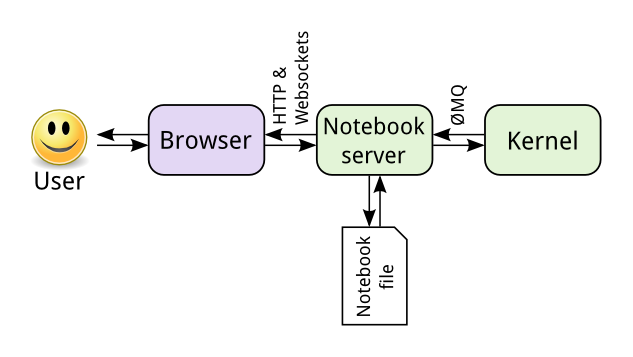
\includegraphics[width=1.0\textwidth]{imagenes/estructurajupyter}
\caption{Estructura de Jupyter Notebook.}
\label{estructurajupyter}
\end{figure}

Los cuadernillos de Jupyter consisten principalmente en dos tipos de celdas: \emph{code} y \emph{markdown}.\emph{ Code }son las celdas ejecutables en las que se escribe código de Python, mientras que \emph{markdown} son las celdas de texto. Para estilizar el texto se usa  la sintaxis de markdown, que permite desde poner texto en negrita hasta insertar imágenes o fórmulas matemáticas complejas.\\

En la Figura \ref{versionjupyter} se pueden var las versiones de los diferentes paquetes necesarios para ejecutar un cuadernillo de Jupyter.

\begin{figure}[h]
\centering
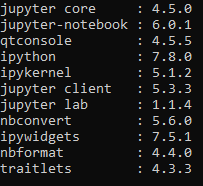
\includegraphics[width=0.5\textwidth]{imagenes/versionjupyter}
\caption{Imagen de una terminal que muestra las versiones de los paquetes de Jupyter usados en este trabajo.}
\label{versionjupyter}
\end{figure}


\section{Prácticas de TDI en Matlab}


Las prácticas originales para la asignatura de Tratamiento Digital de la Imagen consisten en una carpeta zip que se pone a disposición de los alumnos en el aula virtual de la asignatura. Dentro de esta carpeta están las imágenes que se van a utilizar en la práctica (cuando no eran imágenes internas de MatLab), funciones adicionales necesarias en caso de que no existieran previamente y un enunciado en pdf. En la imagen \ref{carpetapracticas} se puede ver un ejemplo de una de estas carpetas.
 
\begin{figure}[h]
\centering
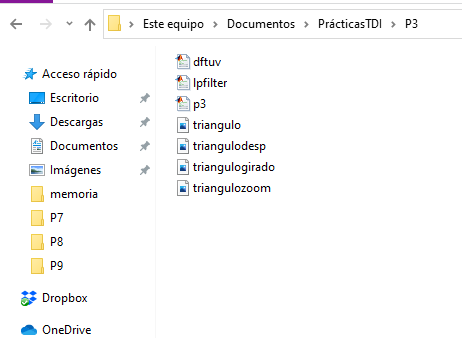
\includegraphics[width=0.5\textwidth]{imagenes/carpetapracticas}
\caption{Ejemplo de carpeta de prácticas.}
\label{carpetapracticas}
\end{figure}

Las prácticas se realizaban en hora de clase en uno de los laboratorios de Windows del campus. Se podían realizar enteras en la duración de la clase. \\

La profesora daba una breve explicación inicial sobre el tema de la práctica, siempre relacionado con lo que se hubiera dado en las clases de teoría recientes. El resto de la práctica se podía seguir de forma libre con el enunciado, con la profesora respondiendo las dudas que surgieran en el desarrollo del ejercicio. \\

Los enunciados son instrucciones detalladas sobre los pasos a seguir para realizar la práctica, con poco o nada de teoría, ya que se asume que el alumno ha recibido las clases de teoría previas. El alumno debe crear un nuevo documento en Matlab e ir ejecutando paso a paso lo que pide el enunciado. \\

Los enunciados suelen comenzar con un breve párrafo explicando el objetivo de la práctica. Por ejemplo en la práctica 4 que trata el tema de segmentación de Imagen, la introducción dice:\emph{``El objetivo de esta práctica es comenzar a familiarizar al alumno con las herramientas básicas de segmentación de imagen en entorno MATLAB. Para ello se trabajará con la imagen en escala de
grises ‘calculadora.tif’, que acompaña al material de esta práctica. "}\\

A partir de esta breve introducción la práctica suele estar dividida en secciones normalmente relacionadas con diferentes puntos tratados en la teoría y cómo llevarlos a cabo.\\

Los pasos a seguir en MatLab, por lo general, vienen dados en el enunciado que indica qué función usar y cómo llamar a las diferentes variables para mantener una consistencia en los nombres a lo largo de la práctica. En algunos casos se indican las variables necesarias para llamar a la función que se va a usar en esa sección del ejercicio, mientras que en otros se pide al alumno que use el comando \textsl{+help} para informarse sobre el funcionamiento de la función. Del mismo modo si una función requiere de un valor a decidir, dependiendo de lo que se quiera conseguir con su uso, unas veces se da con el enunciado y otras se deja a criterio del alumno para que pruebe cómo cambian los resultados con diferentes variables y cuál sería la mejor solución para el problema planteado.\\

Otra característica común de los enunciados de TDI son las preguntas para responder, aunque no se pide una memoria en sí de las prácticas en los enunciados hay preguntas con el objetivo de que el alumno se plantee las respuestas y las razones de los pasos que se han ido realizando durante el ejercicio.  La siguiente imagen \ref{preguntasp4} muestra un ejemplo de estas preguntas del principio de la práctica 4.

\begin{figure}[h]
\centering
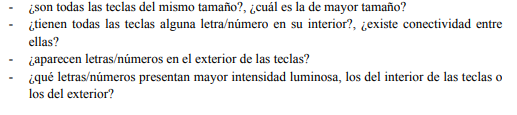
\includegraphics[width=1\textwidth]{imagenes/preguntasp4}
\caption{Ejemplo de preguntas realizadas en los enunciados de TDI.}
\label{preguntasp4}
\end{figure}

Algunos de los enunciados tienen imágenes del aspecto que tendría que tener la imagen sobre la que se está trabajando después de ciertos pasos para que el alumno pueda ver si el ejercicio progresa adecuadamente o si debería modificar alguna variable o revisar el código.\\

Si se pide un algoritmo un poco más complejo, en los enunciados aparece dado un trozo de ese código como ejemplo o directamente para copiar en Matlab ya que el objetivo de estas prácticas no era aprender a programar en MatLab sino ilustrar de forma práctica lo dado en teoría de la asignatura.\\

Las prácticas se suelen centrar en el tratamiento de una imagen en específico, elegida para ilustar el tema del que trata la práctica. Por ejemplo en la práctica 1, en el apartado que trata sobre color se escoge una imagen con diferentes verduras que muestran una variedad de colores para ilustrar la mezcla aditiva de color al representarse individualmente las matrices de cada color del sistema de representación RGB. Debido a que algunas de las imágenes usadas en las prácticas originales pertenecen a Matlab o se desconoce su origen se ha tenido que buscar imágenes nuevas, siempre intentando mantener las características de la imagen original.\\

En total la asignatura consiste de 9 prácticas, 7 de imagen y 2 de video. \\

\begin{itemize}
  \item [ P1.]\emph{Introducción al tratamiento de imagen:}\\
	Esta práctica es una introducción a las herramientas de tratamiento de imagen en Matlab. Se trata cómo leer y representar imágenes, espacios de color, escalado e histogramas. El último apartado se centra en imágenes RGB.
  \item [P2.]\emph{ Filtrado de imágenes en el dominio espacial:}\\
	Esta práctica demuestra el funcionamiento de diferentes tipos de filtros sobre imágenes contaminadas con varios ruidos. En la segunda parte se tratan filtros de realce de contorno y se demuestra su uso para extraer los bordes de unas monedas.
  \item [P3.]\emph{Filtrado de imágenes en el dominio espectral:}\\
	En esta práctica se demuestran las propiedades de la transformada de Fourier y cómo afectan las transformaciones en el espacio a la representación en frecuencia de la imagen. También se tratan filtros en el dominio frecuencial.
  \item [P4.]\emph{Segmentación de imagen:}\\
	Esta práctica es diferente a las anteriores ya que en lugar de ejercicios individuales se centra en el tratamiendo de una imagen en concreto con un objetivo claro. Se trata  la imagen de una calculadora con el objetivo de conseguir una nueva imagen en la que solo se vea la letra Enter de la calculadora. Para esto se usa segmentación binaria que es el tema de la asignatura que se corresponde con esta práctica.
  \item [P5.]\emph{Segmentación de imagen II:}\\
	Esta prácctica sigue el esquema de la anterior centrándose en la segmentación de una imagen, en este caso un pájaro. Para la segmentación de este pájaro se va a usar aprendizaje de máquina, específicamente el algoritmo K-medias, la mayor parte de la práctica se centra en realizar diferentes transformaciones sobre la imagen para facilitar el uso del algoritmo. Entre estas transformaciones se encuentran cambios de espacio de color y filtros de textura.
  \item [P6.]\emph{Morfología binaria:}\\
	Este ejercicio aplica operaciones de morfología matemática para segmentar los chips de una placa y separarlos de acuerdo a su forma.
  \item [P7.]\emph{Segmentación por watershed:}\\
	El objetivo de esta práctica es segmentar una imagen con células para contarlas. Para conseguir esto se plantea el uso del algoritmo de \emph{watershed} con marcadores. Primero se extraen los marcadores internos de las células usando herramientas como la reconstrucción morfológica y conseguir los máximos regionales de una imagen, operaciones estudiadas en la parte correspondiente a esta práctica del temario. Lo mismo ocurre con los marcadores exteriores y el uso de la transformada de distancia. Esta práctica además tiene el objetivo de demostrar que la segmentación de este tipo de elementos que muchas veces se encuentran superpuestos en una imagen es muy complicada y siguen dando bastante error.
  \item [P8]\emph{Manejo de vídeos en MATLAB. Detección y estimación de movimiento:}\\
	Esta es la primera de las prácticas de video, está dividida en dos secciones claras. La primera es una introducción a las herramientas de video en Matlab, estructura de video, como reproducir y guardar videos. La segunda parte trata 3 algoritmos de estimación de movimiento: EBMA, HBMA y correlación de fase.
  \item [P9]\emph{Mejora y restauración de vídeo. Filtrado interfotograma:}\\
	La segunda práctica de vídeo y la última de la asignatura trata la restauración de video contaminado con ruido de una forma muy similar a la práctica 2 de imagen. Primero se centra en el filtrado fotograma a fotograma y después en el filtrado interfotograma, es decir usando varios fotogramas para compararlos entre si y así filtrar.
\end{itemize}

